\documentclass[a4paper,11pt,exos]{nsi} % COMPILE WITH DRAFT
\usepackage{pifont}
\usepackage{fontawesome5}
\usepackage{hyperref}


\pagestyle{empty}


\begin{document}
\classe{\premiere spé}
\titre{Flocon de Von Koch}
\maketitle
On construit une suite de figures géométriques.

\begin{multicols}{5}
    Figure 0 :\\
    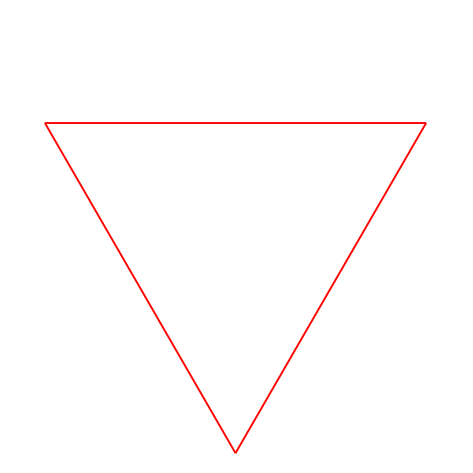
\includegraphics[width=3cm]{Von_Koch0.png}\\
    \vfill\null
    \columnbreak
    Figure 1 :\\
    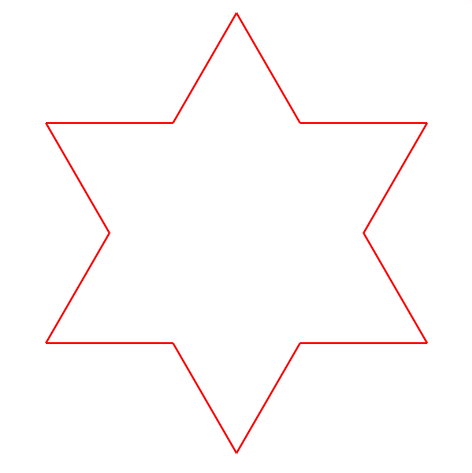
\includegraphics[width=3cm]{Von_Koch1.png}\\
    \vfill\null
    \columnbreak
    Figure 2 :\\
    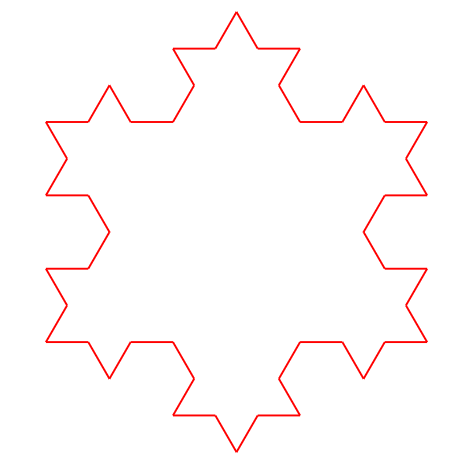
\includegraphics[width=3cm]{Von_Koch2.png}\\
    \vfill\null
    \columnbreak
    Figure 3 :\\
    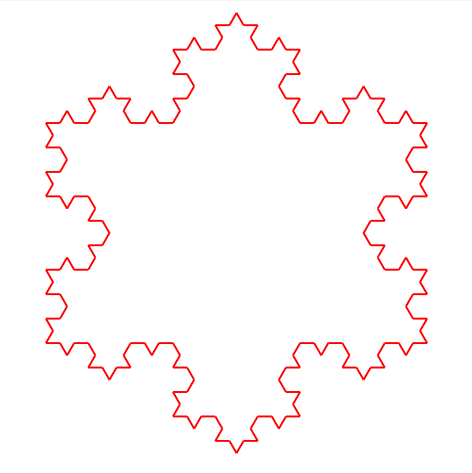
\includegraphics[width=3cm]{Von_Koch3.png}\\
    \vfill\null
    \columnbreak
    Figure 4 :\\
    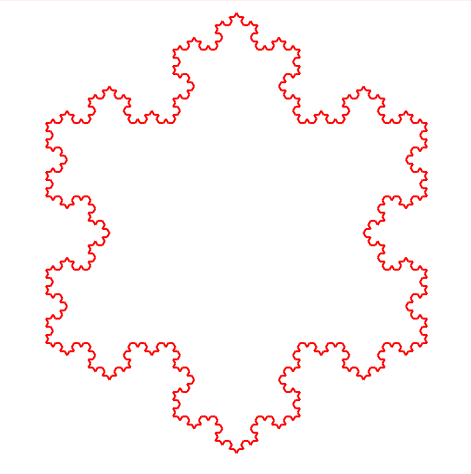
\includegraphics[width=3cm]{Von_Koch4.png}
\end{multicols}

Que pouvez-vous dire :
\begin{enumerate}[label=\textbullet]
    \item Du nombre de côtés de chaque figure ?
    \item De la longueur des côtés de chaque figure ?
    \item De la longueur totale de chaque figure ?
    \item De la l'aire de chaque figure ?
\end{enumerate}

\dleft{14cm}{
    \begin{encadrecolore}{Flocon de Von Koch}{UGLiBlue}
        Lorsque qu'on répète indéfiniment ces étapes, on obtient une courbe appelée \textbf{flocon de Von Koch}.\\
        Cette courbe doit son nom au mathématicien suédois Helge Von Koch qui a l'étudiée en 1904.
    \end{encadrecolore}
}
{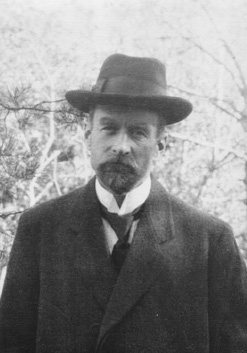
\includegraphics[width=2.3cm]{Helge_von_Koch.jpg}
\begin{center}
    \tiny{Helge Von Koch\\ (1870-1924)}
\end{center}}


\newpage
\titre{Triangle de Sierpinski}
\maketitle
On construit une suite de figures géométriques.

\begin{multicols}{5}
    Figure 0 :\\
    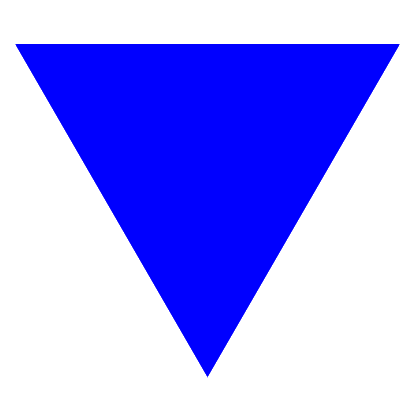
\includegraphics[width=3cm]{Sierpinsky0.png}\\
    \vfill\null
    \columnbreak
    Figure 1 :\\
    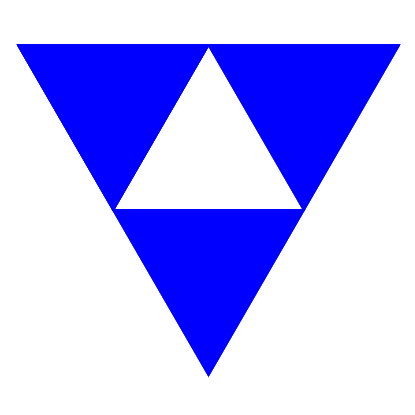
\includegraphics[width=3cm]{Sierpinsky1.png}\\
    \vfill\null
    \columnbreak
    Figure 2 :\\
    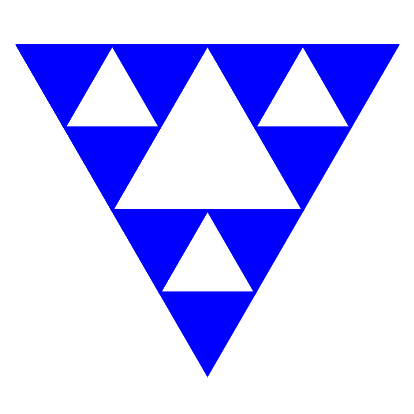
\includegraphics[width=3cm]{Sierpinsky2.png}\\
    \vfill\null
    \columnbreak
    Figure 3 :\\
    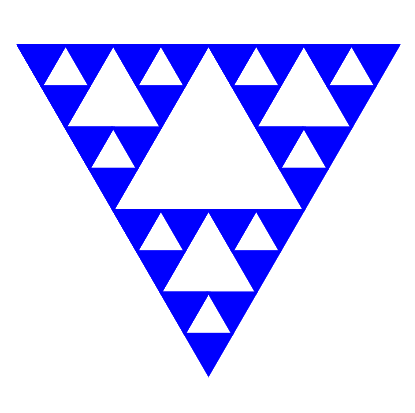
\includegraphics[width=3cm]{Sierpinsky3.png}\\
    \vfill\null
    \columnbreak
    Figure 4 :\\
    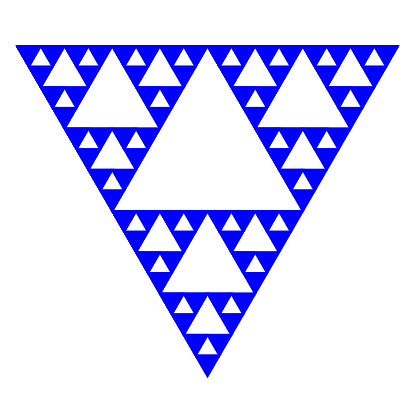
\includegraphics[width=3cm]{Sierpinsky4.png}
\end{multicols}

Que pouvez-vous dire :
\begin{enumerate}[label=\textbullet]
    \item Du nombre de triangle de chaque figure ?
    \item De la longueur des cotés des triangles de chaque figure ?
    \item De la l'aire de chaque figure ?
    \item De la longueur totale du contour de chaque figure ?
\end{enumerate}

\dleft{14cm}{
    \begin{encadrecolore}{Triangle de Sierpinski}{UGLiBlue}
        Lorsque qu'on répète indéfiniment ces étapes, on obtient une surface appelée \textbf{triangle de Sierpinski}.\\
        Cette surface doit son nom au mathématicien polonais Wacław Sierpiński qui a l'étudiée en 1915.
    \end{encadrecolore}
}
{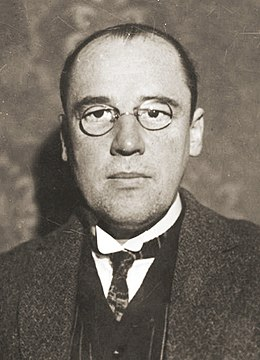
\includegraphics[width=2.3cm]{Wacław_Sierpiński.jpg}
\begin{center}
    \tiny{Wacław Sierpiński\\ (1882-1969)}
\end{center}}

\begin{multicols}{2}
    \begin{center}
        
        
\includegraphics[height=4cm]{Logo-ENPC.svg.png}\\[.5em]
        Logo de l'École Nationale des Ponts et Chaussées\\
        \vfill\null
        \columnbreak
        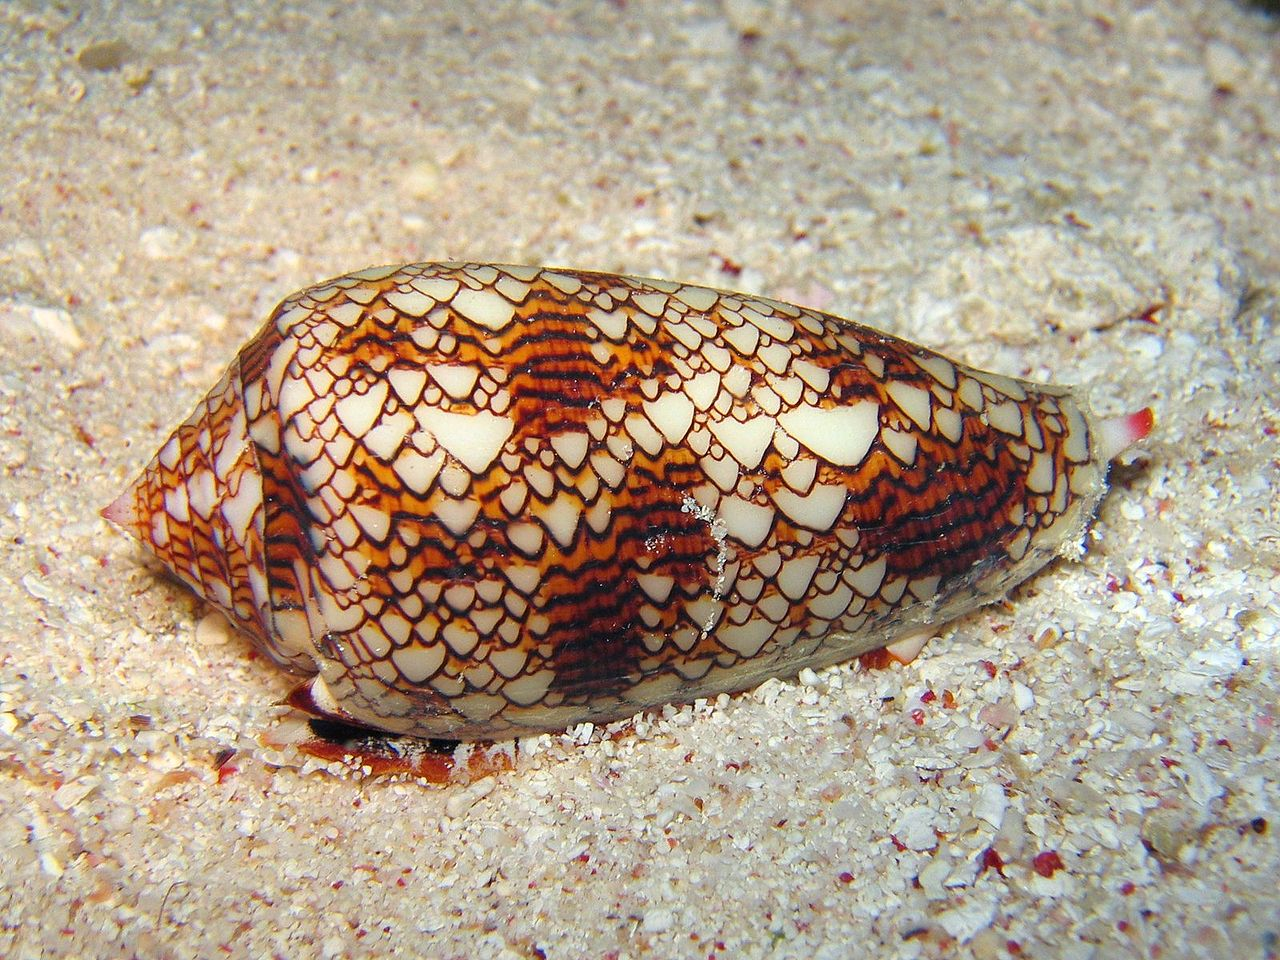
\includegraphics[height=4cm]{Textile_cone.jpg}\\[.5em]
        Motifs de la coquille du Conus textile
    \end{center}
\end{multicols}

\end{document}
